\documentclass[10pt,a4paper,titlepage]{article}
\usepackage[utf8]{inputenc}
\usepackage{amsmath}
\usepackage{amsfonts}
\usepackage{amssymb}
\usepackage[ngerman]{babel}
\usepackage[pdftex]{graphicx}
\usepackage[vmargin=3cm, hmargin=2cm]{geometry}
\usepackage{tabularx}
\usepackage{fancyvrb}

\setlength{\parindent}{0pt}
\setlength{\parskip}{2pt}

\title{Entwurfsdokument}
\author{Simon Bischof \and Jan Haag \and Adrian Herrmann \and Lin Jin \and Tobias Schlumberger \and Matthias Schnetz}

\makeindex

\begin{document}

\thispagestyle{empty}
\vspace*{4cm}
\begin{center}
\begin {huge}
Entwurfsdokument\\
\end{huge}
Simon Bischof, Jan Haag, Adrian Herrmann, Lin Jin, Tobias Schlumberger, Matthias Schnetz\\
\vspace{3cm}
\begin{huge}
Praxis der Softwareentwicklung \\
Projekt 3:\\
Automatisches Pr\"{u}fen der Korrektheit von Programmen\\
Gruppe 1\\
\vspace{2cm}

\includegraphics[height=2cm]{images/Logo.pdf}\\[0.5cm]
\end{huge}
\begin{huge}
WS 2011/2012
\end{huge}
\end{center}
\newpage
\tableofcontents
\newpage

\section{Einleitung}

\section{Klassendiagramme}

\subsection{"Ubersicht}

Das folgende Klassendiagramm zeigt die Grobstruktur der Anwendung. \\
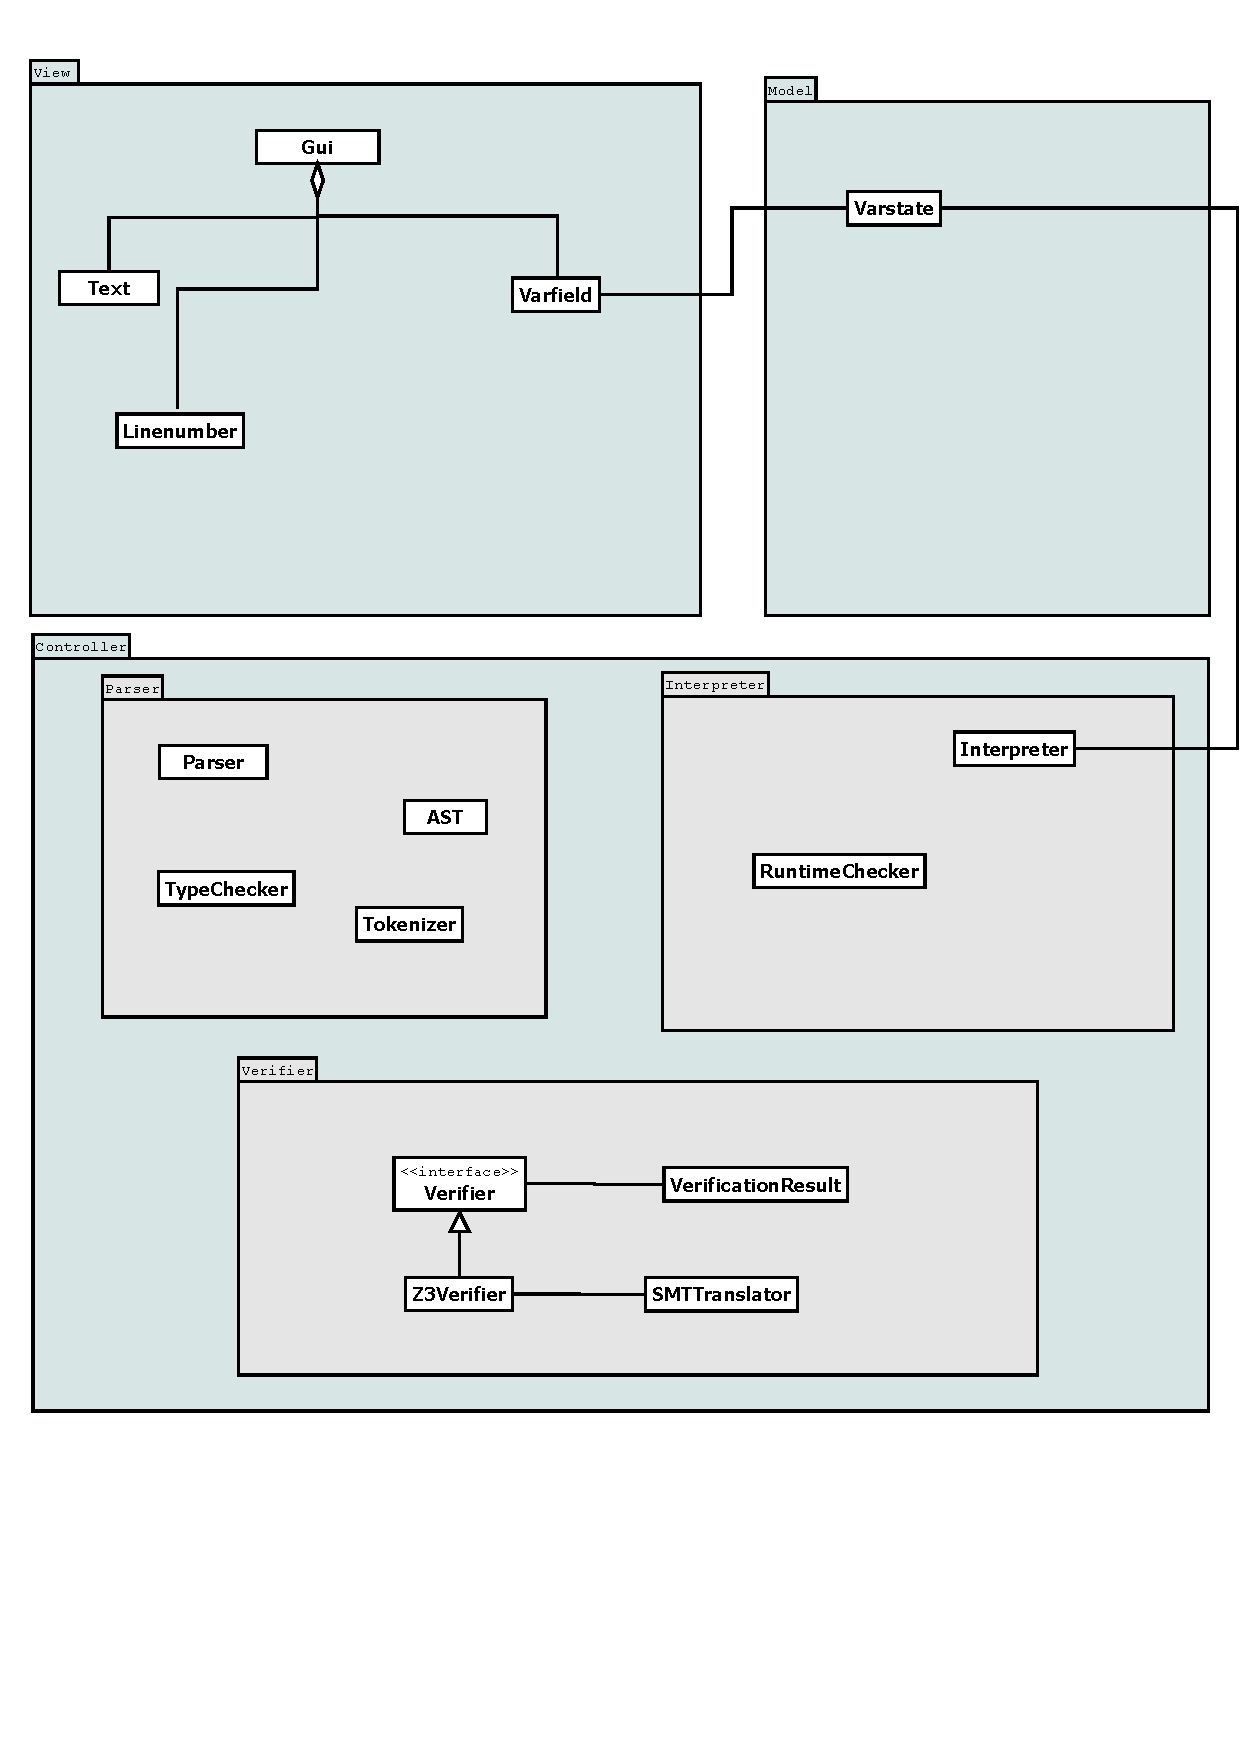
\includegraphics[scale=0.8]{images/ClassOverview.pdf} \\
Die gesamte Architektur basiert auf dem Entwurfsmuster Model-View-Controller. Dies erm"oglicht uns einen flexiblen Programmentwurf, der eine sp"atere "Anderung oder Erweiterung erleichtert und eine Wiederverwendbarkeit der einzelnen Komponenten erm"oglicht.
\begin{itemize}
\item Das \textbf{Modell} enth"alt die darzustellenden Daten, z.B die Zust"ande der Variablen w"ahrend der Programmausf"uhrung und die vom Benutzer gesetzten Breakpoints
\item Die \textbf{Pr"asentation/View} stellt die Daten aus dem Modell auf der Benutzeroberfl"ache dar und nimmt Benutzerinteraktionen entgegen
\item Um die Zusammenarbeit der ersten zwei Komponenten k"ummert sich die \textbf{Steuerung}. Au"serdem f"uhrt sie die Hauptaktionen (Parsen, Interpretieren, usw.) aus und bearbeitet die Eingaben des Benutzers \\\\
\end{itemize}

\subsection{Feinstruktur der Komponenten}

\subsubsection{Programmstruktur}

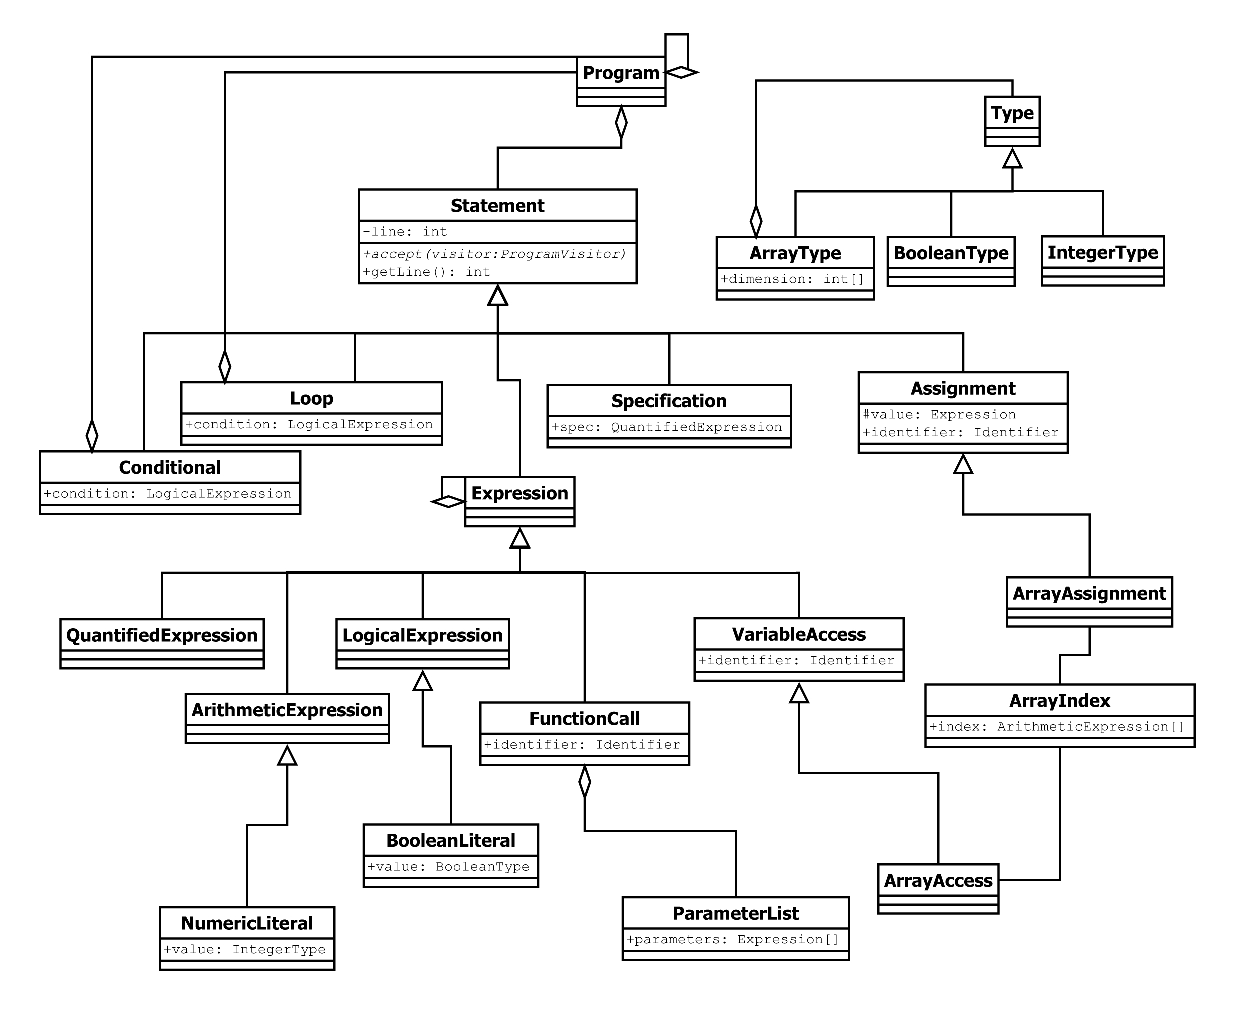
\includegraphics[scale=0.85]{images/AST.pdf} \\
F"ur die Struktur des AST verwenden wir das Composite-Muster. Damit wird die Teil-Ganzes-Hierachie der While-Grammatik repr"asentiert, indem Objekte zu Baumstrukturen zusammengef"ugt werden. Au"sdem erm"oglicht uns das Muster, Objekte und Kompositionen einheitlich zu behandeln. 
\begin{itemize}
\item \texttt{Program} \\
Die Klasse \texttt{Program} stellt eine Funktion im Quelltext dar. 
\begin{itemize}
\item Attribute: \\
\texttt{program} \\
eine Instanz von sich selbst. Diese sind Unterprogramme, die aufgerufen werden k"onnen.\\
\texttt{statement} \\
eine Liste von Instanzen der Klasse \texttt{Statement}
\end{itemize}
\item \texttt{Statement} \\
Die abstrakte Klasse \texttt{Statement} steht f"ur eine Anweisung des Programms. Die Anweisungen sind eingeteilt in f"unf Klassen: \texttt{Conditional, Loop, Specification, Assignment} und \texttt{Expression}. 
\begin{itemize}
\item Attribut:\\
\texttt{line} \\
Zeile im Quelltext, in der sich die Instanz befindet
\item Methoden: \\
\texttt{getLine()} \\
gibt das Attribut \texttt{line} zur"uck \\
\texttt{\textit{accept(visitor: ProgramVisitor)}}\\
abstrakte Methode, die von den Unterklassen implementiert wird
\end{itemize}
\item \texttt{Conditional} \\
Die Klasse \texttt{Conditional} steht f"ur eine bedingte Anweisung. 
\begin{itemize}
\item Attribute: \\
\texttt{program} \\
Unterprogramme, die bedingt ausgef"uhrt werden \\
\texttt{condition} \\
Bedingung, die "uberpr"uft wird
\end{itemize}
\item \texttt{Loop} \\
Die Klasse \texttt{Loop} steht f"ur eine while-Anweisung. 
\begin{itemize}
\item Attribute: \\
\texttt{program} \\
Unterprogramme, die bedingt ausgef"uhrt werden \\
\texttt{condition} \\
Bedingung, die "uberpr"uft wird
\end{itemize}
\item \texttt{Specification}
\begin{itemize}
\item Attribut: \\
\texttt{spec} \\
Ausdruck, der "uberpr"uft wird
\end{itemize}
\item \texttt{Assignment} \\
Die Klasse \texttt{Assignment} steht f"ur eine Zuweisung von Variablen. Die Klasse \texttt{ArrayAssignment} ist eine Subklasse, die stattdessen f"ur Zuweisung von Arrays steht.
\begin{itemize}
\item Attribute: \\
\texttt{value} \\
der Wert, der zugewiesen wird\\
\texttt{identifier} \\
die Variable, der \texttt{value} zugewiesen wird
\end{itemize}
\item \texttt{Expression} \\
Die abstrakte Klasse \texttt{Expression} steht f"ur einen beliebigen Ausdruck. \texttt{QuantifiedExpression}, \\
\texttt{ArithmeticExpression, LogicalExpression, FunctionCall} und \texttt{VariableAccess} sind Unterklassen dieser Klasse.
\item \texttt{FunctionCall} \\
Die Klasse \texttt{FunctionCall} modelliert einen Methodenaufruf. 
\begin{itemize}
\item Attribute: \\
\texttt{identifier} \\
Name der Methode \\
\texttt{paralist} \\
Liste von Parametern, die der Methode "ubergeben werden
\end{itemize}
\item \texttt{VariableAccess} \\
Die Klasse \texttt{VariableAccess} stellt einen Zugriff auf eine vorhandene Variable dar. Von dieser Klasse erbt die Unterklsse \texttt{ArrayAccess}. 
\begin{itemize}
\item Attribut: \\
\texttt{identifier} \\
Name der Variable 
\end{itemize}
\item \texttt{Type} \\
Die Klasse \texttt{Type} bildet eine Oberklasse der verschiedenen Typen, die eine Variable haben kann. Dazu geh"oren \texttt{BooleanType}, \texttt{IntegerType} und \texttt{ArrayType}.
\item \texttt{ArrayType} \\
Die Klasse \texttt{ArrayType} definiert einen eigenen Typ der Array-Objekte. 
\begin{itemize}
\item Attribute: \\
\texttt{dimension} \\
Dimension des Arrays \\
\texttt{type} \\
Arrayelemente haben "`normale"' Typen \\
\end{itemize}
\end{itemize}

\subsubsection{Besucherklassen}

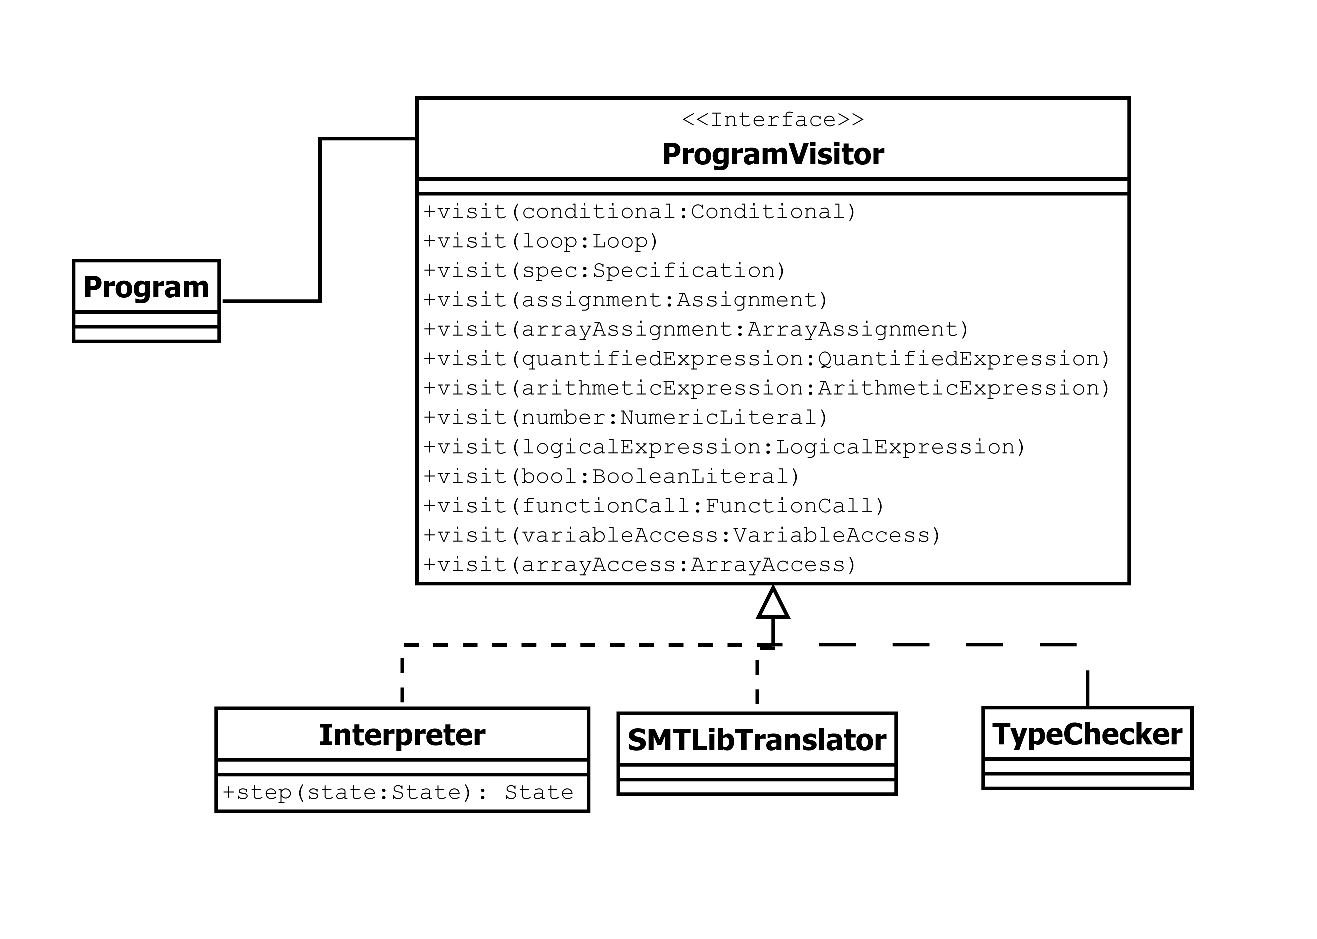
\includegraphics[scale=0.7]{images/Besucher.pdf} \\
F"ur die Integration der verschiedenen Methoden, wie zum Beispiel die des Interpreters, verwenden wir das Visitor-Muster. Es kapselt die Operationen, die auf Elemente des AST ausgef"uhrt werden. Das Muster erm"oglicht uns, Operationen zu ver"andern oder neue Funktionen hinzuf"ugen, ohne die Elementklassen zu modifizieren. 
\begin{itemize}
\item \texttt{ProgramVisitor} \\
Das Interface \texttt{ProgramVisitor} deklariert f"ur jede Klasse konkreter Elemente eine Besuchsfunktion.
\item \texttt{Interpreter} \\
Die Klasse \texttt{Interpreter} ist ein konkreter Besucher und implementiert die Aufgaben des Interpretierens als Besuchsfunktionen. 
\begin{itemize}
\item Methode: \\
\texttt{step(state:State)} \\
schrittweise Ausf"uhrung des Programms. Dabei wird der Funktion der aktuellen Zustand \texttt{state} "ubergeben und diese gibt wieder eine Instanz der Klasse \texttt{State} zur"uck. \\
\end{itemize}
\end{itemize}

\subsubsection{Parser}

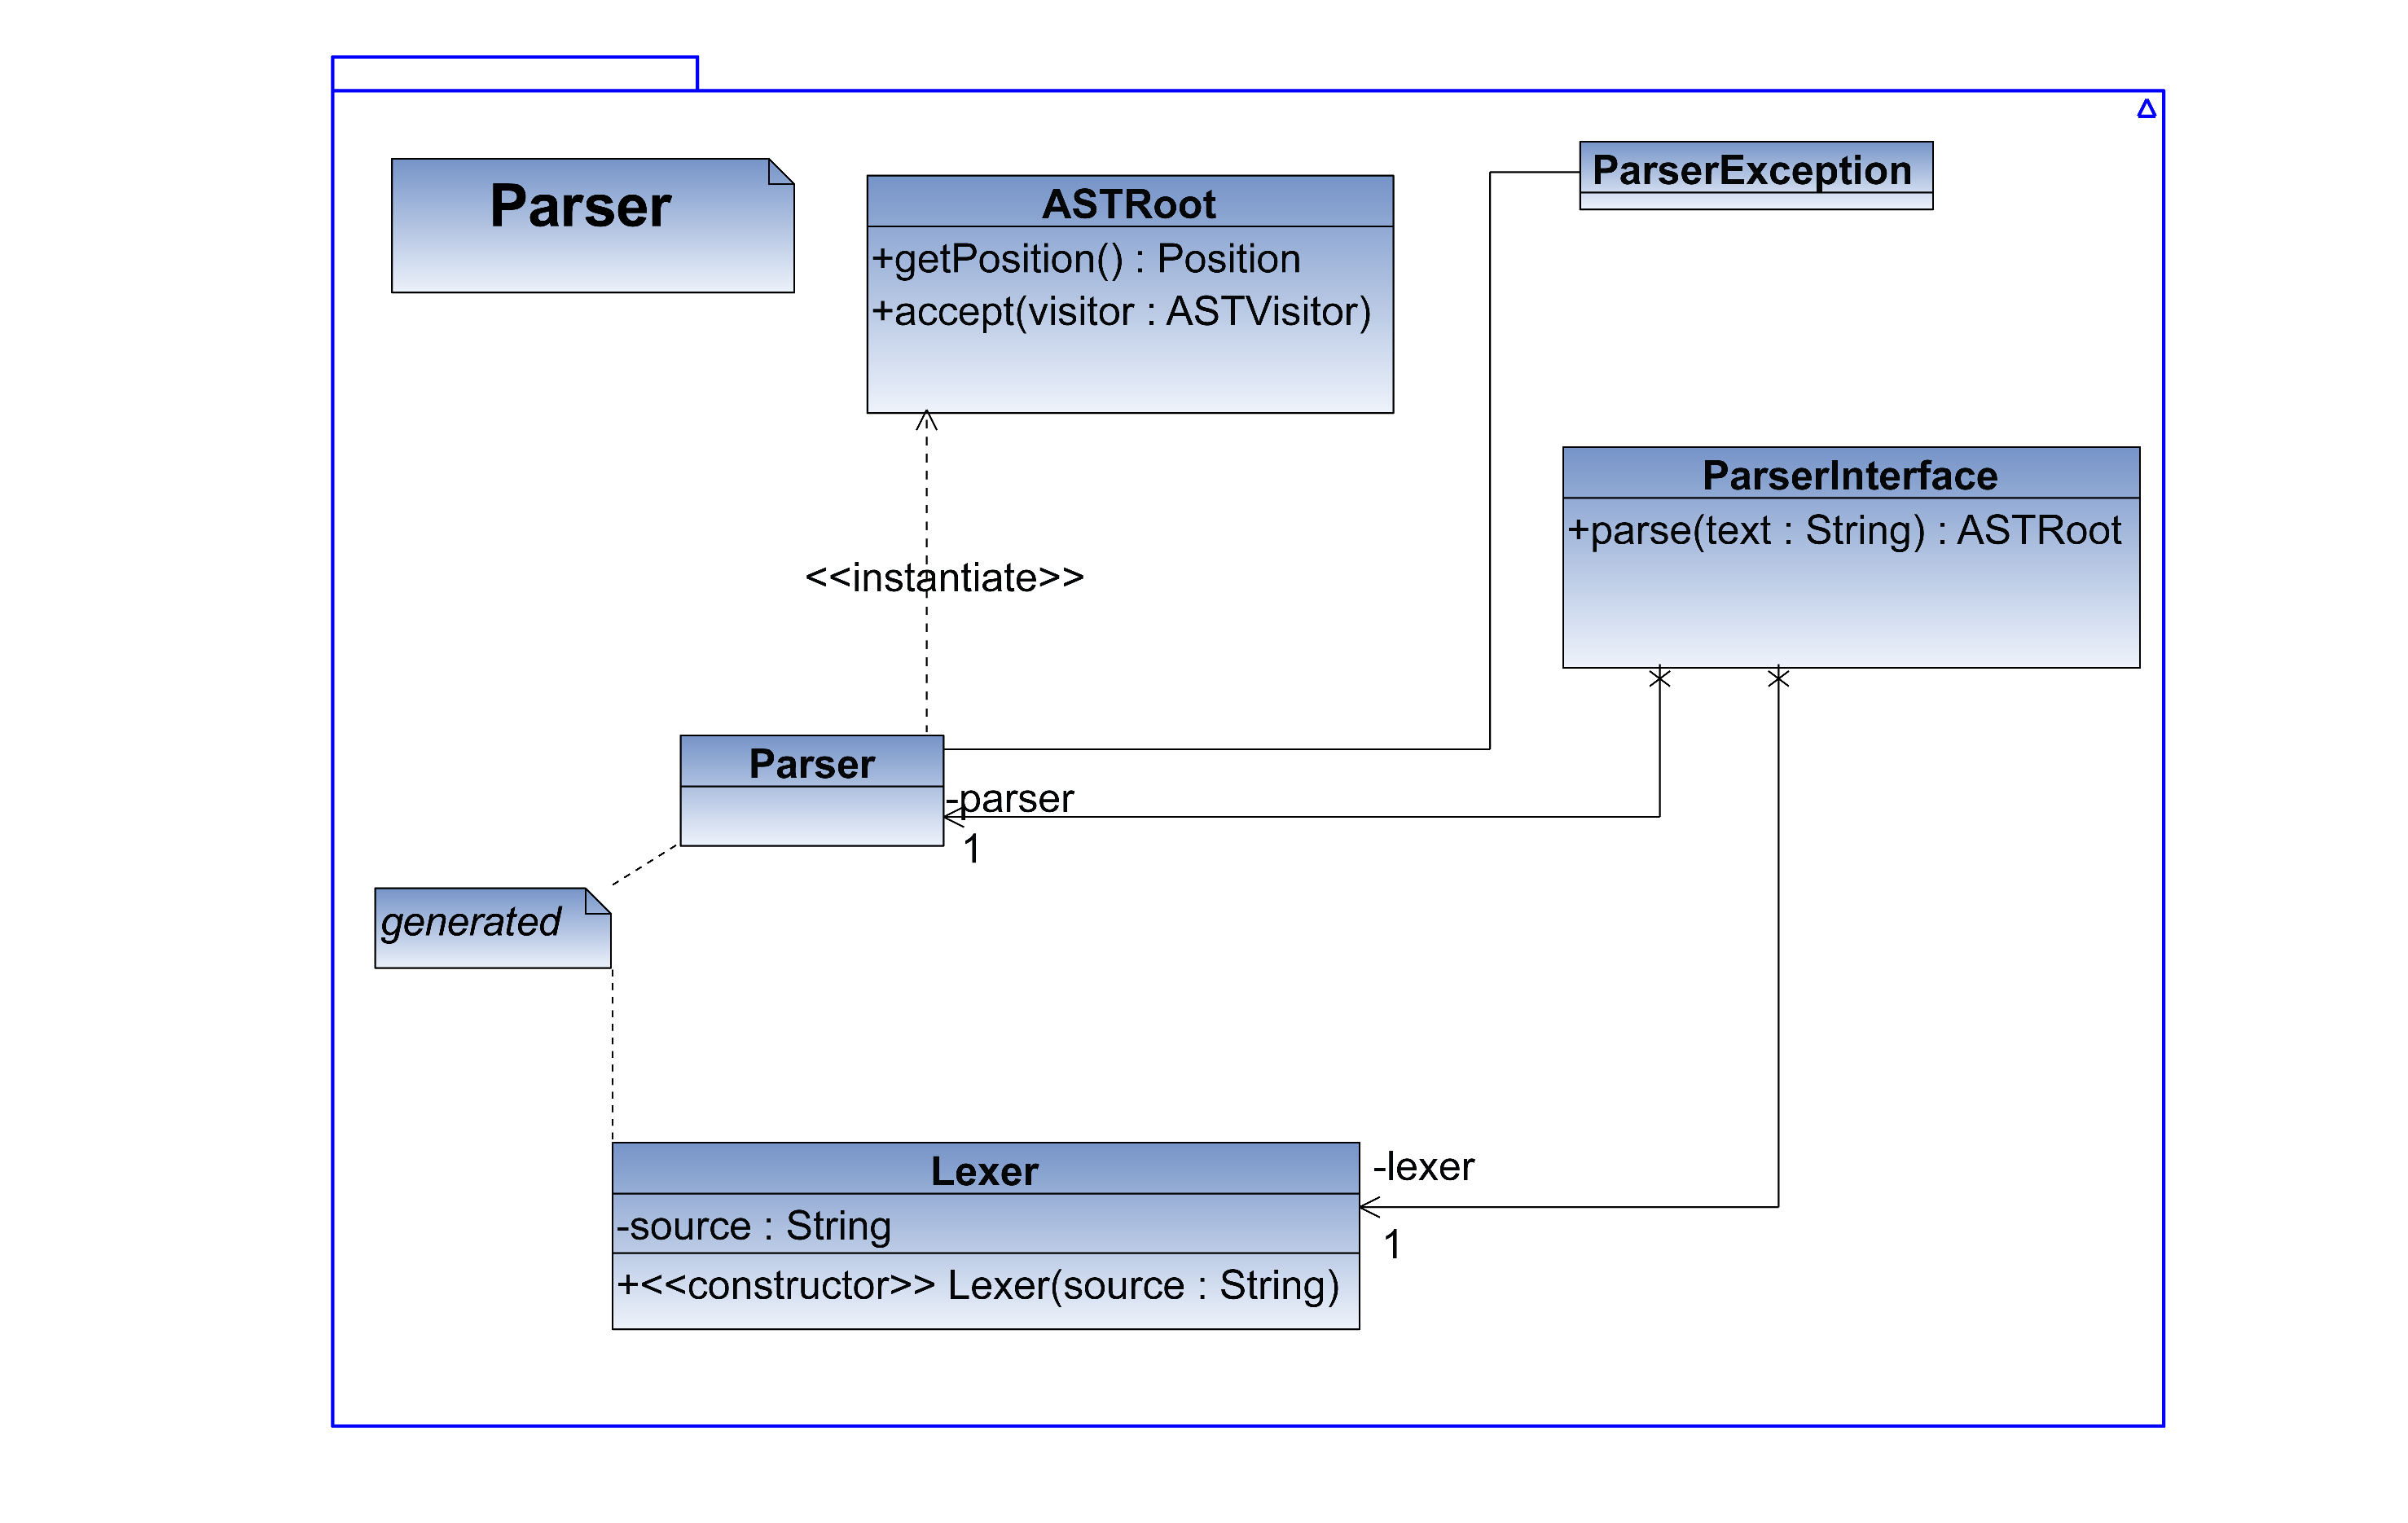
\includegraphics[scale=0.5]{images/Parser.pdf} \\
Die Klassen der Komponente Parser werden vom Parsergenerator ANTLR erstellt. Der Parser liefert die Struktur des AST. 
\begin{itemize}
\item \texttt{Lexer} \\
Die Klasse \texttt{Lexer} zerlegt den Quelltext in Tokens. 
\begin{itemize}
\item Attribut: \\
\texttt{source} \\
der vom Benutzer eingegebene Quelltext 
\item Methoden: \\
\texttt{Lexer(source:String)} \\
Konstruktor der Klasse. Bei der Instanzierung wird der Quelltext "ubergeben. \\
\texttt{getSource()} \\
gibt den Quelltext zur"uck \\
\end{itemize}
\end{itemize}

\subsubsection{Modell}

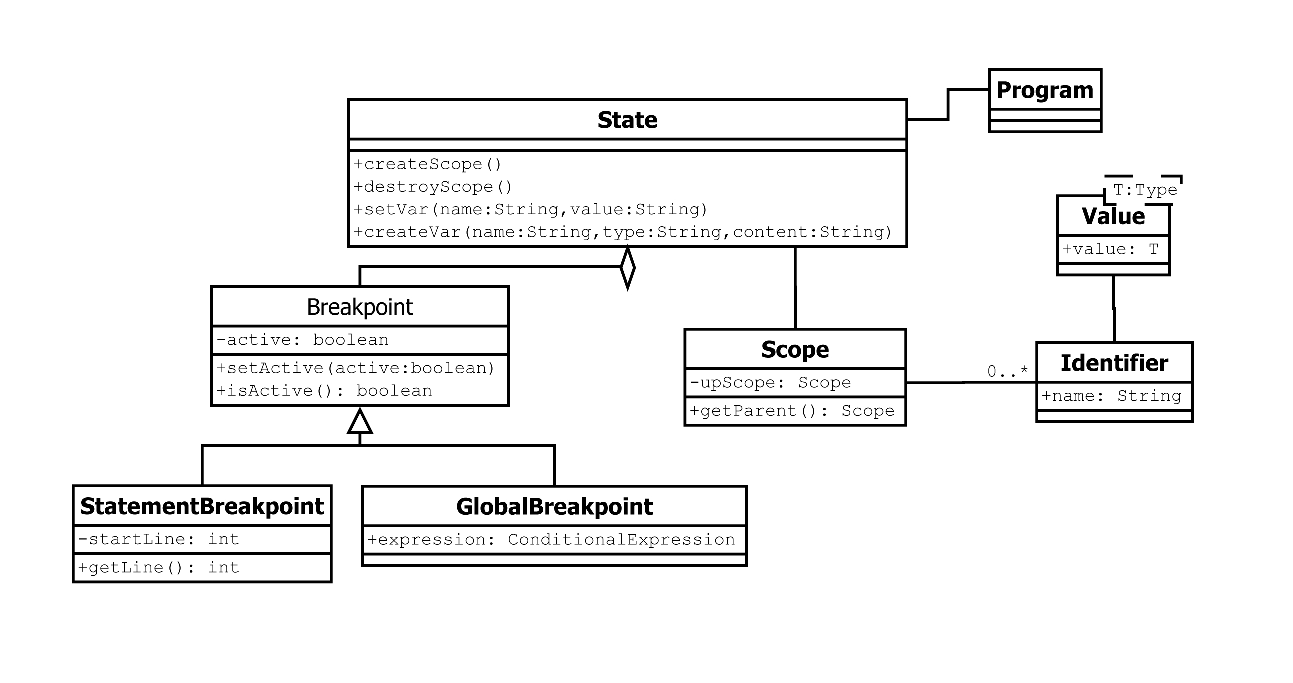
\includegraphics[scale=0.8]{images/Modell.pdf} \\
Die Komponente Modell speichert alle Daten der Anwendung. Diese erh"alt sie von den Komponenten View (z.B. Benutzereingaben) und Controller (z.B. Zustand der Programmausf"uhrung). Au"serdem ist es ihre Aufgabe, Daten auf Anforderung der anderen Komponenten bereit zustellen. 
\begin{itemize}
\item \texttt{Scope} \\
Die Klasse \texttt{Scope} bildet eine Hierachie der Sichtbarkeit von Variablen des Programms. Je weiter unten sich eine \texttt{Scope}-Instanz befindet, desto lokaler ist die damit verbundenen Variable. In der obersten Ebene befinden sich also die globalen Variablen. Bei einem Variablenzugriff wird zun"achst die unterste Ebene "uberpr"uft, ob diese die gesuchte Variable enth"alt. Wenn dies nicht der Fall ist, so sucht man in der n"achst h"oheren Ebene weiter. Wenn man bereits die oberste Ebene erfolglos durchsucht hat, ist die Variable nicht vorhanden und eine Exception wird geworfen. 
\begin{itemize}
\item Attribute: \\
\texttt{upScope} \\
eine andere Instanz der Klasse, die in der Hierachie "uber diese Instanze liegt \\
\texttt{identifier} \\
Name der Variable, deren Sichtbarkeit durch diese Instanz dargestellt wird
\item Methode: \\
\texttt{getParent()} \\
gibt die "`Eltern"'-Instanz \texttt{upScope} zur"uck
\end{itemize}
\item \texttt{Value} \\
Die Klasse \texttt{Value} speichert den Wert einer zugeh"origen Variable. 
\begin{itemize}
\item Attribute: \\
\texttt{value} \\
Attribut mit einem generischen Typ, der BooleanType, IntegerType oder ArrayType sein kann. 
\texttt{identifier} \\
Name der Variable, die den Wert \texttt{value} besitzt
\end{itemize}
\item \texttt{State} \\
Die Klasse \texttt{State} speichert den aktuellen Zustand der Programmausf"uhrung, wie z.B. Werte von Variablen. Au"serdem ordnet sie den Variable ihre Sichtbarkeit zu.
\begin{itemize}
\item Methoden: \\
\texttt{createScope()} \\
erzeugt f"ur eine Variable die entsprechende \texttt{Scope}-Instanz \\
\texttt{destroyScope()} \\
zerst"ort eine \texttt{Scope}-Instanz \\
\texttt{setVar(name:String,value:String)}  \\
setzt eine Variable und ihren Wert mithilfe eines Stringinputs \\
\texttt{createVar(name:String,type:String,content:String} \\
erstellt eine Variable mit Typ und Inhalt mithilfe eines Stringinputs 
\end{itemize}
\item \texttt{Breakpoint} \\
Die abstrakte Klasse \texttt{Breakpoint} hat zwei Subklassen: \texttt{StatementBreakpoint} und \texttt{GlobalBreakpoint}. 
\begin{itemize}
\item Attribut: \\
\texttt{active} \\
boolsche Variable, die anzeigt, ob die \texttt{Breakpoint}-Instanz aktiviert ist 
\item Methoden: \\
\texttt{setActive(active:boolean)} \\
aktiviert oder deaktiviert diese \texttt{Breakpoint}-Instanz \\
\texttt{isActive()} \\
gibt \texttt{active} zur"uck
\end{itemize}
\item \texttt{StatementBreakpoint} \\
Die Klasse \texttt{StatementBreakpoint} stellt einen an einer Zeile gebundenen Breakpoint dar. 
\begin{itemize}
\item Attribut: \\
\texttt{startLine} \\
Zeile, in der sich der Breakpoint befindet
\item Methode: \\
\texttt{getLine()} \\
gibt \texttt{startLine} zur"uck
\end{itemize}
\item \texttt{GlobalBreakpoint}
Die Klasse \texttt{GlobalBreakpoint} stellt einen globalen Breakpoint dar, der an einem Ausdruck gebunden ist. 
\begin{itemize}
\item Attribut: \\
\texttt{expression} \\
Ausdruck, an dem die Instanz gebunden ist \\
\end{itemize}
\end{itemize}

\subsubsection{Benutzeroberfl"ache}

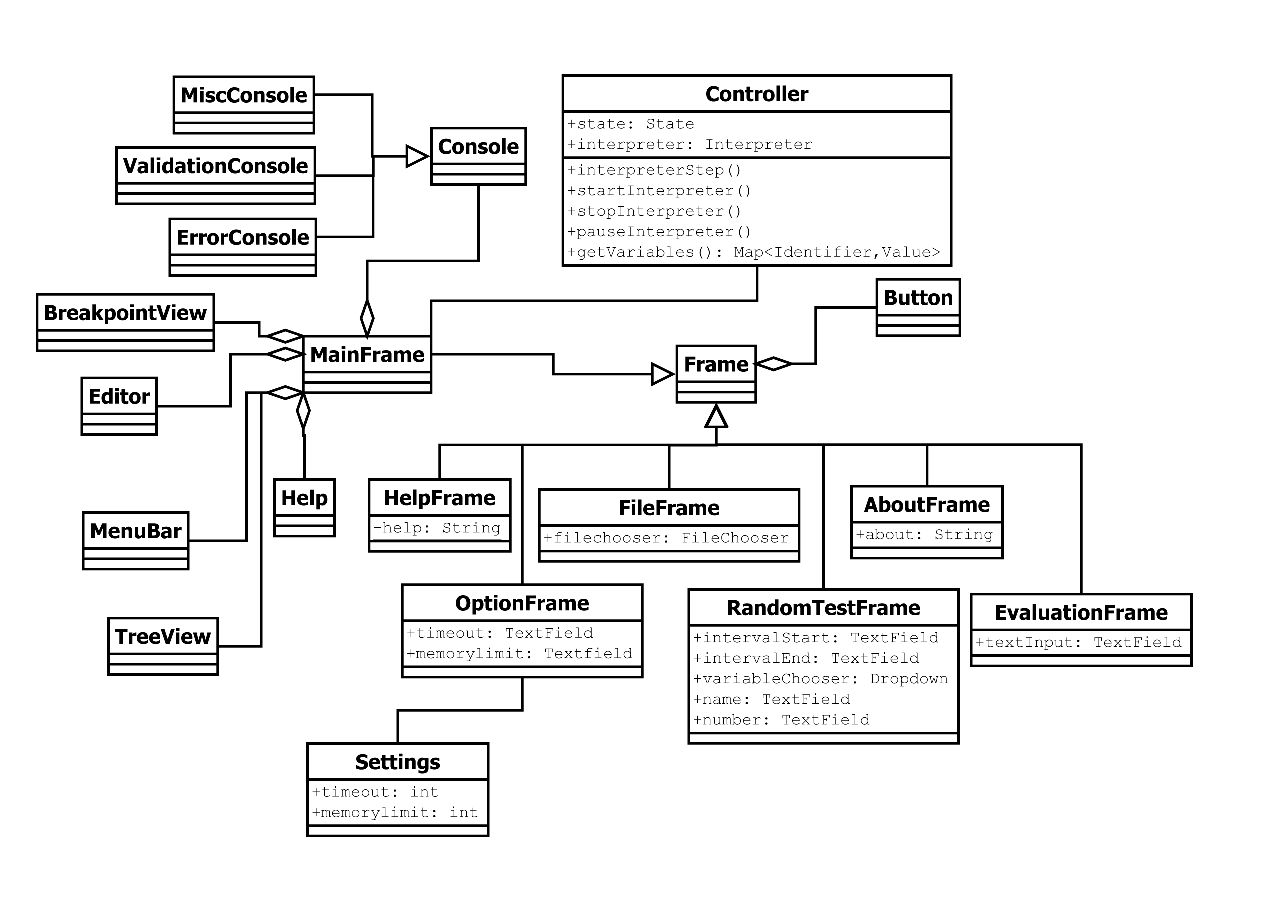
\includegraphics[scale=0.85]{images/GUI.pdf} \\
Die Benutzeroberfl"ache bietet dem Benutzer eine leicht zu bedienende Schnittstelle und nimmt dessen Eingaben entgegen. Um eine flexible Struktur zu gestalten, verwenden wir hier das Facade-Muster in Form der \texttt{Controller}-Klasse. Diese vereinfacht die Schnittstelle zu den restlichen Komponenten und f"ordert die lose Kopplung. "Uber sie geschehen alle Interaktionen mit anderen Komponenten, z.B. reicht sie Benutzereingaben weiter, damit diese verarbeitet werden k"onnen. Der \texttt{Controller} stellt der GUI auch die von ihr ben"otigten Informationen zur Verf"ugung. 
\begin{itemize}
\item \texttt{Controller} \\
Die Klasse \texttt{Controller} stellt eine Verbindung zwischen dem Modell und der View her. 
\begin{itemize}
\item Attribute: \\
\texttt{state} \\
Zustand des Programms \\
\texttt{interpreter} \\
die \texttt{Interpreter}-Instanz, die das aktuelle Programm ausf"uhrt 
\item Methoden: \\
\texttt{interpreterStep()} \\
schrittweise Ausf"uhrung des Programms \\
\texttt{startInterpreter()} \\
Ausf"uhrung des gesamten Programms \\
\texttt{stopInterpreter()} \\
Ausf"uhrung abbrechen \\
\texttt{pauseInterpreter()} \\
Ausf"uhrung pausieren \\
\texttt{getVariables()} \\
gibt die aktuellen Variablen und deren Werte zur"uck 
\end{itemize}
\item \texttt{Frame} \\
Die abstrakte Klasse \texttt{Frame} stellt alle Fenster dar, die vom Benutzer ge"offnet werden k"onnen. Sie ist Oberklasse der folgenen Klassen: \texttt{HelpFrame, FileFrame, OptionFrame, RandomTestFrame, AboutFrame, EvaluationFrame} und \texttt{MainFrame}.
\item \texttt{HelpFrame} \\
Die Klasse \texttt{HelpFrame} erleichtert die Bedienung der Anwendung. 
\begin{itemize}
\item \texttt{help} \\
Inhalt der Hilfe 
\end{itemize}
\item \texttt{OptionFrame} \\
Die Klasse \texttt{OptionFrame} speichert Benutzereinstellungen f"ur den Beweiser. 
\begin{itemize}
\item Attribut: \\
\texttt{settings} \\
in der \texttt{Settings}-Instanz sind die vom Benutzer festgelegte Werte f"ur \texttt{timeout} und \texttt{memorylimit} gespeichert
\end{itemize}
\item \texttt{MainFrame} \\
Die Klasse \texttt{MainFrame} ist das Hauptfenster der Benutzeroberfl"ache. Sie besteht aus einem \texttt{Editor}, einer \texttt{MenuBar}, einer \texttt{BreakpointView}, einer \texttt{TreeView}, mehreren \texttt{Console}s und einem \texttt{Help}-Fenster. 
\begin{itemize}
\item Attribut: \\
\texttt{controller} \\
vereinfachte Schnittstelle, leitet Funktionalit"aten weiter \\
\end{itemize}
\end{itemize}

\newpage

\section{Aktivit"atsdiagramme}

\subsection{Parser/Type-Checker}

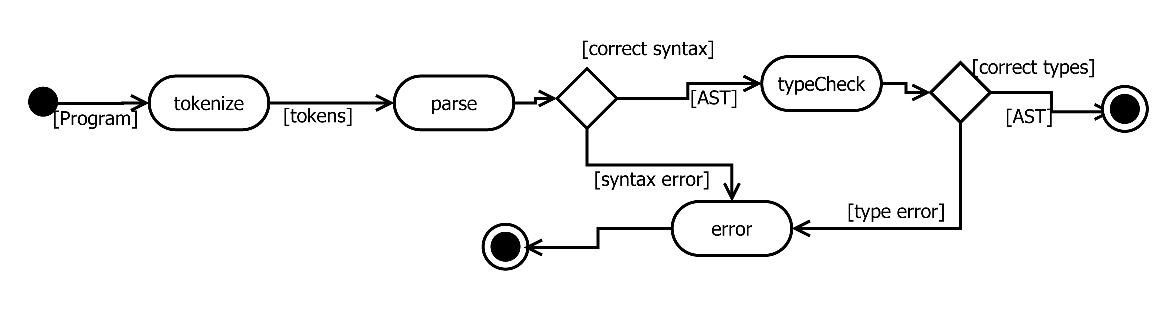
\includegraphics[scale=0.8]{images/AktivitaetParser.pdf}\newline
Beim Aufruf des Interpreters wird das Programm in mehreren Schritten geparst.
\begin{enumerate}
\item Der Programmtext wird als einzelner String dem Tokenizer "ubergeben.
\item Der Tokenizer trennt den String an den wichtigen Stellen und gibt ein Array von Tokens zur"uck.
\item Der Parser generiert bei syntaktisch korrekten Programmen daraus einen abstrakten Syntaxbaum (AST).
\item Bei Syntaxfehlern bricht der Parser mit einem Fehler ab.
\item Im Erfolgsfall "uberpr"uft der Typechecker die Korrektheit der Typen: Sind die Typen korrekt, gibt dieser den vom Parser generierten AST zur"uck, sonst beendet er sich mit einem Fehler.
\end{enumerate}

\subsection{Z3-Anbindung}

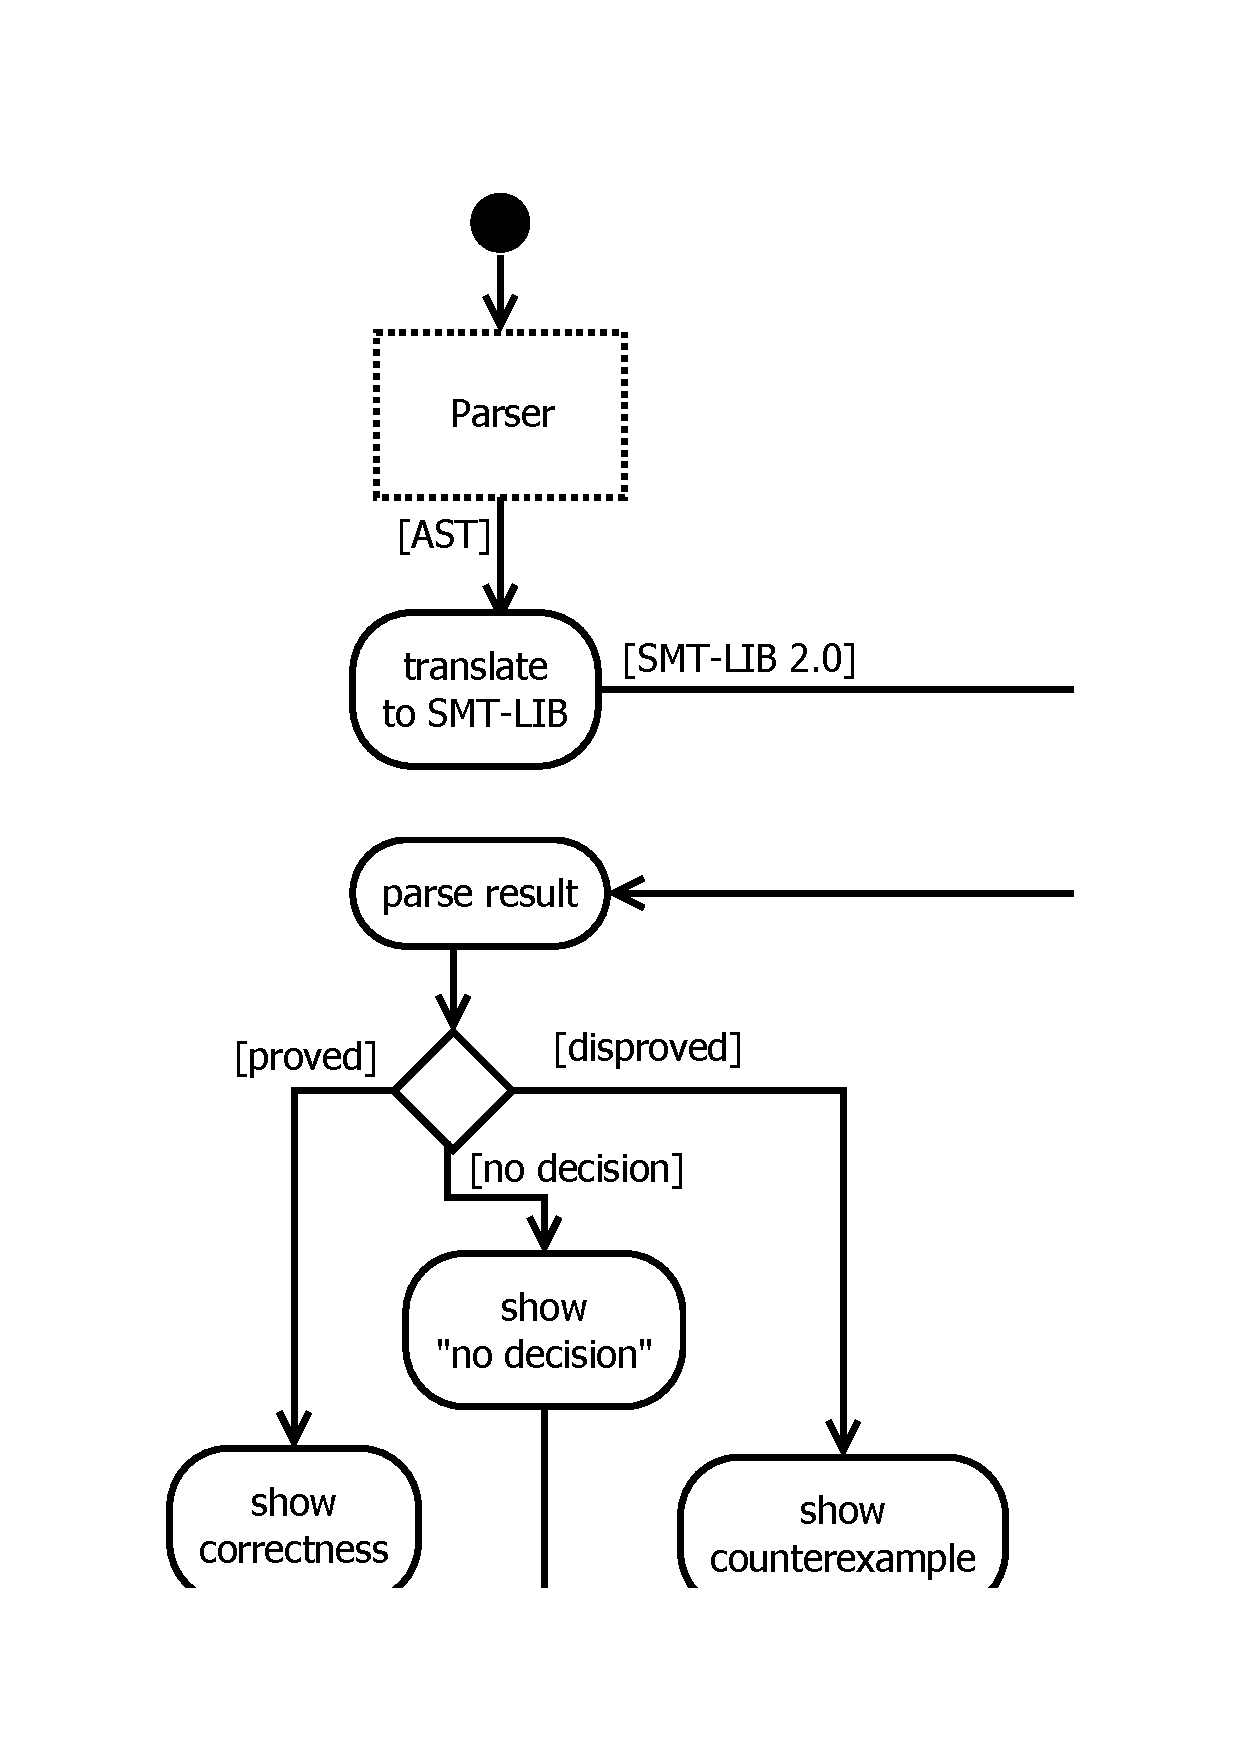
\includegraphics[scale=0.5]{images/AktivitaetSMTTranslator.pdf}\\\\
Zur "uberpr"ufung der Korrektheit des Programms wird Z3 benutzt. 
\begin{enumerate}
\item Zuerst wird das Programm geparst (siehe Aktivit"atsdiagramm Parser/Type-Checker).
\item Im Fehlerfall ist keine "Uberpr"ufung durch Z3 m"oglich. Im Erfolgsfall wird der durch den Parser generierte AST an den SMTLib-Translator gegeben.
\item Der SMTLib-Translator "ubersetzt das Programm inklusive Spezifikation ins SMTLib-2.0-Format. Dieses bildet die Eingabe f"ur Z3.
\item Die von Z3 zur"uckgegebene Antwort wird vom Result-Parser analysiert.
\item Meldet der Beweiser die Korrektheit des Programms oder konnte er keine Entscheidung treffen, wird dieses Ergebnis dem Benutzer bekannt gegeben. Falls der Beweiser das Programm falsifizieren konnte, wird dem Benutzer das Ergebnis zusammen mit einem m"oglichen Gegenbeispiel angezeigt.
\end{enumerate}

\section{Zustandsdiagramm}

Das folgende Zustandsdiagramm zeigt das Verhalten des Systems bei Benutzeraktionen. \\
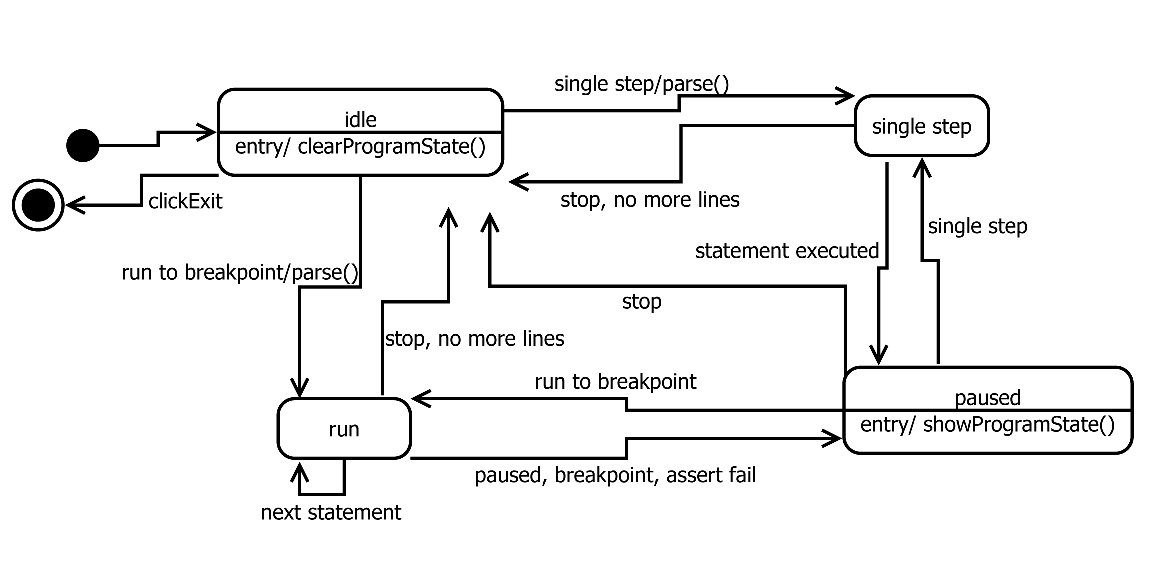
\includegraphics[scale=0.9]{images/Zustand.pdf}
\begin{itemize}
\item Beim Starten des Programms geht dieses in den "`idle"'-Zustand. Hier l"auft der Interpreter nicht, und es ist kein Programmzustand gespeichert. Falls einer vorhanden ist, wird dieser beim Eintritt in den "`idle"'-Zustand gel"oscht.
\item Beim Ausw"ahlen von "`single step"' wird das Userprogramm geparst und ein Statement wird ausgef"uhrt, nachdem der Zustand "`single step"' betreten worden ist. Ist kein Statement mehr vorhanden, so beendet sich der Interpreter, das Programm geht zur"uck in den Zustand "`idle"'. Sonst wird nach Ausf"uhren des Statements das Programm pausiert, der Zustand "`paused"' wird eingenommen.
\item Beim Eintritt in den "`paused"'-Zustand wird der Zustand des Userprogramms ausgegeben. W"ahrend der Pausierung l"auft der Interpreter nicht. In diesem Zustand stehen die gleichen M"oglichkeiten wie im "`idle"'-Zustand zu Verf"ugung, das Parsen bei Verlassen des Zustands entf"allt aber.
\item Wenn im "`idle"'-Zustand "`run to breakpoint"' aufgerufen wird, wird das Userprogramm geparst und das Programm geht in den Zustand "`run"'. Das Userprogramm wird solange ausgef"uhrt, bis es zu Ende ist (neuer Zustand: "`idle"') oder der Interpreter pausiert, ein Breakpoint getroffen oder eine Assertion falsifiziert wird. In diesen F"allen ist der neue Zustand "`paused"'.
\item In jedem Zustand au"ser "`idle"' ist es zus"atzlich m"oglich, das Userprogramm abzubrechen, wobei der Interpreter beendet wird und alle vorhandenen Variablen-Informationen gel"oscht werden. Das Programm geht danach in den Zustand "`idle"'.
\item In jedem Zustand kann das Programm durck einen Klick auf den Exit-Button beendet werden.
\end{itemize}
\newpage

\section{Struktur der While-Sprache}
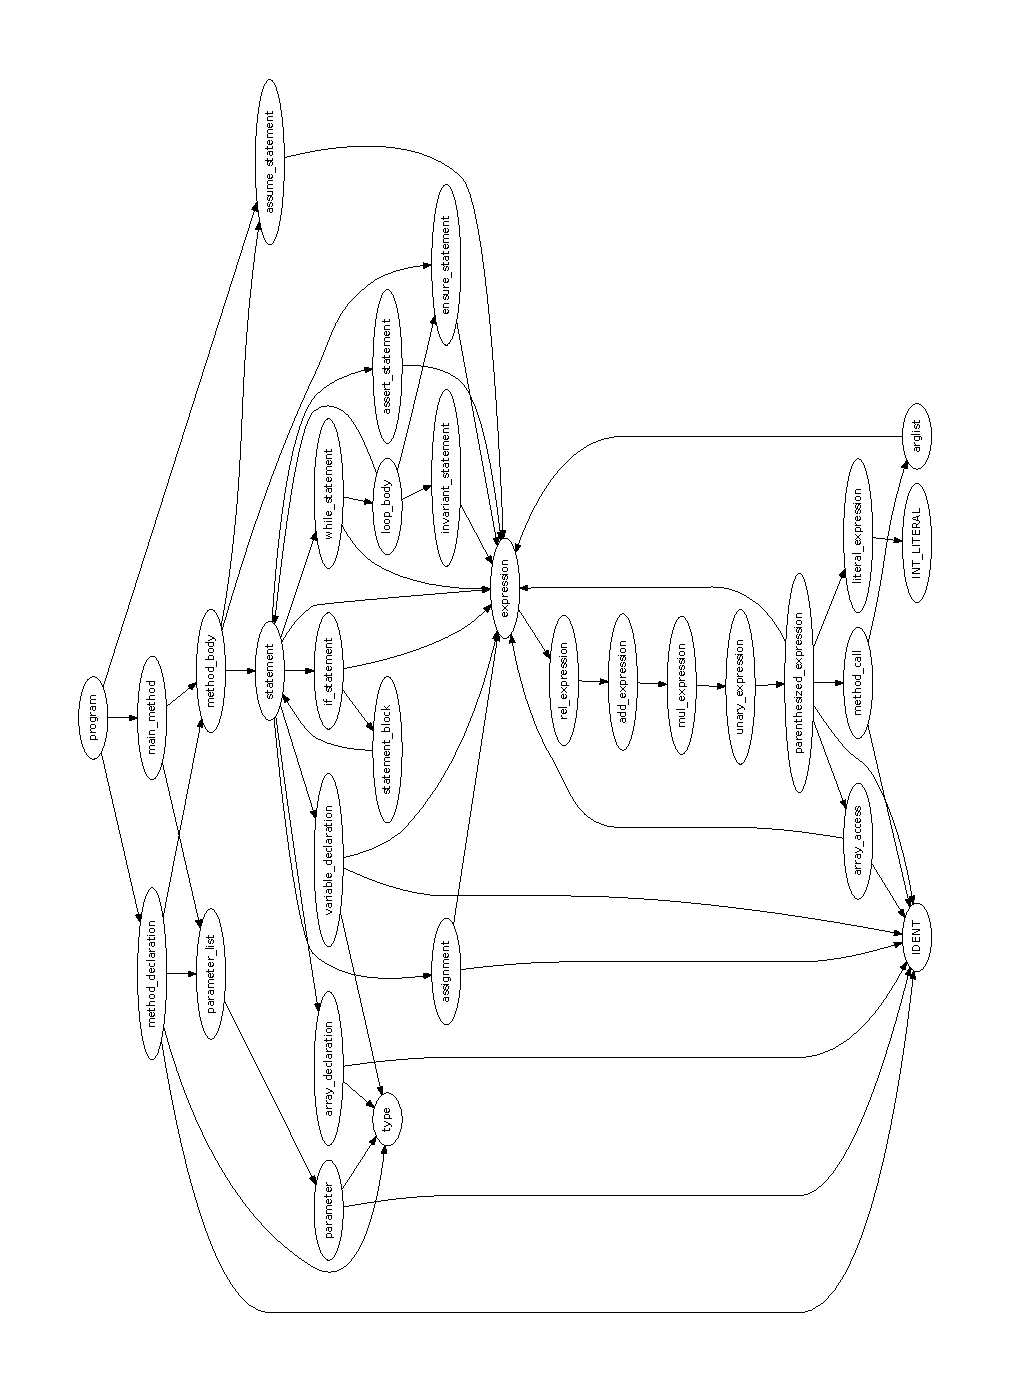
\includegraphics[scale=1]{images/DependencyGraph.pdf}

\section{Syntax der While-Sprache}
\VerbatimInput{WhileLanguage.g}
\end{document}

